\chapter{Proper Time, Time Dilation, and Length Contraction}

This lecture, though delivered inside the entanglement track, is really a special-relativity lecture. These notes follow Leonard Susskind's order of attack as preserved in the LazyingArt LLC course curation: start with Galileo, correct the kinematics so that light has the same speed for everybody, then use the resulting spacetime geometry to understand proper time, time dilation, the twin paradox, signal exchange, and finally length contraction. The argument is deliberately picture-first. We are not handed isolated formulas; we are shown why each one appears when it does.

\section{Review: Galilean Relativity and Its Spacetime Grid}

Susskind begins by fixing a practical convention. Sometimes the speed of light will be written explicitly as \(c\), and sometimes it will be set equal to \(1\). We will follow that convention. Most of the algebra is cleaner in units with \(c=1\), and whenever dimensions matter we can restore the missing factors of \(c\) by dimensional analysis.

The pre-Einsteinian starting point is Galilean relativity. For motion along a single spatial direction,
\begin{align}
x' &= x-vt, &
t' &= t.
\end{align}
This is Newton's world. The moving origin drifts through space, but time is universal. If we solve for the unprimed coordinates, we find
\begin{align}
x &= x'+vt = x'+vt', &
t &= t'.
\end{align}
The structure is reciprocal: going from one observer to the other only reverses the sign of the velocity.

Susskind phrases the story in train-and-station language. He imagines himself on the moving train and the audience at rest on the platform, while also reminding us that the whole point of relativity is that either side may regard itself as the one at rest. But before Einstein is allowed to enter, one wants to see exactly what Galileo would have drawn.

The first geometric fact is that the moving observer's spatial origin is the locus \(x'=0\). In the unprimed coordinates this becomes
\begin{equation}
x=vt \iff x'=0.
\end{equation}
That line is the \(t'\)-axis, drawn on the same \((x,t)\) graph as the original axes. The line tilts because the moving origin drifts, but the constant-time slices do not. Since \(t'=t\), a surface of constant \(t'\) is also a surface of constant \(t\). In Galilean relativity all observers share the same simultaneity.

\begin{figure}[h]
\centering

\includegraphics[width=0.56\textwidth]{lecture_04_figure_02.png}

\vspace{1em}

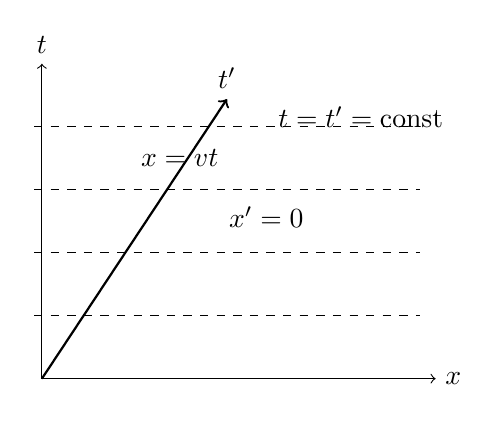
\begin{tikzpicture}[x=1cm,y=1cm]
\draw[->] (0,0) -- (0,4) node[above] {$t$};
\draw[->] (0,0) -- (5,0) node[right] {$x$};
\draw[thick,->] (0,0) -- (2.35,3.55) node[above] {$t'$};

\draw[dashed] (-0.1,0.8) -- (4.8,0.8);
\draw[dashed] (-0.1,1.6) -- (4.8,1.6);
\draw[dashed] (-0.1,2.4) -- (4.8,2.4);
\draw[dashed] (-0.1,3.2) -- (4.8,3.2);

\node at (1.75,2.8) {$x=vt$};
\node at (2.85,2.05) {$x'=0$};
\node at (4.05,3.32) {$t=t'=\mathrm{const}$};
\end{tikzpicture}
\caption{The board at the start of the Galilean review, followed by a clean reconstruction of the spacetime picture described immediately afterward in the lecture. The moving origin traces the slanted line \(x=vt\), but the constant-time slices remain horizontal because \(t'=t\).}
\end{figure}

This is the baseline. Einstein's correction will be intelligible only if we keep this old grid in view.

\section{From Galileo to Lorentz}

The reason the Galilean formulas fail is equally simple and equally profound: they are inconsistent with the statement that the speed of light is the same in every inertial frame. The corrected formulas are the Lorentz transformations. In units with \(c=1\),
\begin{align}
x' &= \frac{x-vt}{\sqrt{1-v^2}}, &
t' &= \frac{t-vx}{\sqrt{1-v^2}}.
\end{align}
Restoring dimensions gives
\begin{align}
x' &= \frac{x-vt}{\sqrt{1-v^2/c^2}}, &
t' &= \frac{t-vx/c^2}{\sqrt{1-v^2/c^2}}.
\end{align}

Susskind makes two immediate points. First, for everyday velocities the correction is negligible:
\begin{equation}
\sqrt{1-\frac{v^2}{c^2}} \approx 1
\qquad\text{when}\qquad
v \ll c.
\end{equation}
So Newtonian physics survives as the low-velocity approximation. Special relativity is not a repudiation of Galileo; it is the refinement that becomes necessary when \(v\) approaches \(c\).

Second, the really new feature is not the denominator in \(x'\) but the fact that \(t'\) is no longer equal to \(t\). Newton believed in a universal time shared by everyone. Einstein's formula says that once the speed of light is universal, time itself must mix with space.

There is also a directional asymmetry built into the formula. If the relative motion is along the \(x\)-axis, then the transverse coordinates are unchanged:
\begin{equation}
y'=y, \qquad z'=z.
\end{equation}
Only the coordinate along the direction of motion gets entangled with time.

Susskind also pauses on the denominator. When \(v\) approaches \(c\), the factor \(\sqrt{1-v^2/c^2}\) tends to zero. The algebra is warning us that one inertial frame cannot move at exactly the speed of light relative to another. Long before one reaches that point, however, measurable deviations from Galilean intuition begin to appear.

\subsection{Question \& Answer}

\paragraph{Question.} Why do \(y\) and \(z\) stay unchanged while \(x\) mixes with \(t\)? And what is the real invariant content of the transverse meter-stick argument?

\paragraph{Answer.} The lecture's answer is operational and symmetrical. Imagine two meter sticks oriented transversely to the motion, one carried on the train and one at rest on the platform. Consider an observer halfway between the two frames, a bicyclist in Susskind's language, who sees them approaching with equal and opposite velocities. In that halfway frame the setup is completely symmetric. There is no reason for one transverse rod to pass the other looking shorter. So the transverse directions cannot contract.

But the deeper point is about events. When two endpoints meet, that meeting is a spacetime coincidence. One may mark it by a flash of light, but the flash is only evidence; the coincidence itself is the event. If two events occur at the same spacetime point in one frame, they occur at the same spacetime point in every frame. Thus the transverse rod argument is not merely a visual story. It rests on the invariance of events.

\section{Light-Cone Coordinates and the Geometry of Lorentz Transformations}

At this point Susskind deliberately changes the way he looks at the formulas. He says, in effect: let me show you another way to write the Lorentz transformation. First he gets rid of the \(c\)'s, because they are a nuisance for the algebra, and then he adds and subtracts the two equations.

Adding the transformed coordinates gives
\begin{align}
t'+x'
&= \frac{(t-vx)+(x-vt)}{\sqrt{1-v^2}} \\
&= \frac{(t+x)(1-v)}{\sqrt{1-v^2}} \\
&= (t+x)\sqrt{\frac{1-v}{1+v}}.
\end{align}
Subtracting gives
\begin{align}
t'-x'
&= \frac{(t-vx)-(x-vt)}{\sqrt{1-v^2}} \\
&= \frac{(t-x)(1+v)}{\sqrt{1-v^2}} \\
&= (t-x)\sqrt{\frac{1+v}{1-v}}.
\end{align}

This is not merely algebraic housekeeping. The combinations
\begin{equation}
t+x, \qquad t-x
\end{equation}
are coordinates along the two \(45^\circ\) null directions in a spacetime diagram with \(c=1\). In other words, they are adapted to the light cone itself. Under a Lorentz transformation, each of these null coordinates is simply rescaled, and the two scale factors are inverses of one another.

That is the geometric content Susskind wants us to see. A Lorentz transformation is a squeeze: one lightlike direction is stretched while the other is compressed by the reciprocal amount. The crucial thing is what does \emph{not} change. The \(45^\circ\) directions remain \(45^\circ\). Light rays stay light rays. That is precisely the geometric meaning of the principle that the speed of light is frame-independent.

Once one sees the Lorentz transformation this way, the next question presents itself almost automatically. If the transformation squeezes spacetime but leaves the light cone intact, what quantity does it preserve?

\section{Proper Time as the Invariant Interval}

Before he writes down the formula, Susskind does something wise. He explains what kind of object proper time is supposed to be. Imagine a collection of stationary observers, each carrying a synchronized clock. Their network defines a coordinate time. Now imagine one observer moving through that network with a wristwatch. The wristwatch does not carry the whole stationary grid along with it; it carries only its own ticking. Proper time will be the time read by that moving clock.

With that operational picture in the background, Susskind turns to the geometric analogue of Euclidean distance. For ordinary rotations in the plane, the invariant quantity is
\begin{equation}
s^2=x^2+y^2=x'^2+y'^2.
\end{equation}
Under a Lorentz transformation, the corresponding invariant is different by a minus sign:
\begin{equation}
t'^2-x'^2=t^2-x^2.
\end{equation}

\begin{proposition}
Under the Lorentz transformation in \(1+1\) dimensions, the quantity \(t^2-x^2\) is invariant.
\end{proposition}

\begin{proof}
Starting from
\begin{equation}
x'=\frac{x-vt}{\sqrt{1-v^2}},
\qquad
t'=\frac{t-vx}{\sqrt{1-v^2}},
\end{equation}
we compute
\begin{align}
t'^2-x'^2
&= \frac{(t-vx)^2-(x-vt)^2}{1-v^2} \\
&= \frac{t^2-2tvx+v^2x^2-x^2+2xvt-v^2t^2}{1-v^2} \\
&= \frac{(1-v^2)t^2-(1-v^2)x^2}{1-v^2} \\
&= t^2-x^2.
\end{align}
The cross terms cancel, and the common factor \(1-v^2\) drops out.
\end{proof}

In three spatial dimensions the corresponding statement is
\begin{equation}
t'^2-x'^2-y'^2-z'^2=t^2-x^2-y^2-z^2.
\end{equation}
The lecture mostly works along one axis, but this fuller expression makes clear that the invariant does not care which spatial direction we happened to choose for the relative motion.

\begin{definition}
If one event is the origin and a second event lies in the time-like region, its proper time from the origin is
\begin{equation}
\tau=\sqrt{t^2-x^2}
\end{equation}
in units with \(c=1\). More generally, one applies the same invariant to coordinate differences between two events:
\begin{equation}
\Delta \tau^2=\Delta t^2-\Delta x^2-\Delta y^2-\Delta z^2.
\end{equation}
\end{definition}

Why the square root? Because the analogy is with ordinary distance. In Euclidean geometry the distance between two points is the square root of the invariant quadratic form. Here the invariant quadratic form has a minus sign in the spatial directions, but the logic is the same.

Now the sign difference begins to matter. If \(t^2>x^2\), the quantity under the square root is positive and the proper time is real. If \(t^2=x^2\), the proper time is zero. If \(t^2<x^2\), the separation is space-like, and in the lecture Susskind says bluntly that the proper time is imaginary. The polished statement is that space-like separated points are not related by ordinary elapsed clock time, but his warning is useful: Minkowski geometry is not Euclidean geometry with a new accent; the minus sign changes everything.

\begin{figure}[h]
\centering
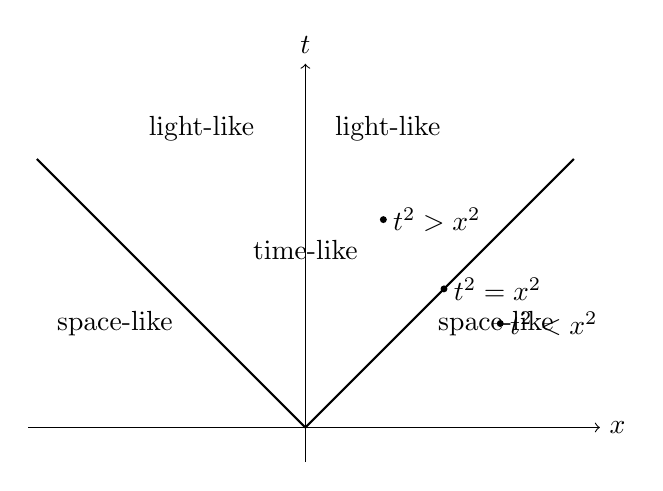
\begin{tikzpicture}[x=1.1cm,y=1.1cm]
\draw[->] (-3.2,0) -- (3.4,0) node[right] {$x$};
\draw[->] (0,-0.4) -- (0,4.2) node[above] {$t$};

\draw[thick] (0,0) -- (3.1,3.1);
\draw[thick] (0,0) -- (-3.1,3.1);

\node at (0.95,3.45) {light-like};
\node at (-1.2,3.45) {light-like};
\node at (0,2.05) {time-like};
\node at (2.2,1.2) {space-like};
\node at (-2.2,1.2) {space-like};

\fill (0.9,2.4) circle (0.04);
\fill (1.6,1.6) circle (0.04);
\fill (2.25,1.2) circle (0.04);

\node[right] at (0.9,2.4) {$t^2>x^2$};
\node[right] at (1.6,1.6) {$t^2=x^2$};
\node[right] at (2.25,1.2) {$t^2<x^2$};
\end{tikzpicture}
\caption{The light cone in \(1+1\) dimensions. Inside the cone the interval is time-like and the proper time is real; on the cone the proper time is zero; outside the cone the separation is space-like.}
\end{figure}

The operational interpretation now falls into place. For a clock at rest in the unprimed frame, \(x=0\), so
\begin{equation}
\tau=\sqrt{t^2}=t.
\end{equation}
Thus proper time agrees with ordinary time for an observer at rest.

For a moving clock, we may always transform to the frame in which the clock is momentarily at rest. Along that worldline \(x'=0\), and so
\begin{equation}
\tau=\sqrt{t'^2-x'^2}=t'.
\end{equation}
This is the heart of the lecture's definition: moving clocks tick off proper time. The invariant interval is not just a formula that everyone agrees on; it is the quantity that the traveling wristwatch actually reads.

\section{Time Dilation and Relativity of Simultaneity}

Now Susskind uses proper time as a tool. Consider the simplest possible moving worldline: the origin of the primed frame itself. In the unprimed coordinates this worldline is
\begin{equation}
x=vt \iff x'=0.
\end{equation}
So the slanted line in the spacetime diagram is not merely a particle trajectory. It is the moving observer's time axis.

\begin{figure}[h]
\centering

\includegraphics[width=0.54\textwidth]{lecture_04_figure_03.png}

\vspace{1em}

\begin{tikzpicture}[x=1cm,y=1cm]
\draw[->] (0,0) -- (0,4) node[above] {$t$};
\draw[->] (0,0) -- (5,0) node[right] {$x$};

\draw[thick,->] (0,0) -- (2.35,3.6) node[above] {$t'$};
\node at (1.45,2.85) {$x=vt$};
\node at (3.05,2.0) {$x'=0$};

\fill (1.75,2.68) circle (0.04);
\draw[dashed] (1.75,2.68) -- (0,2.68);
\node[left] at (0,2.68) {$t$};
\end{tikzpicture}
\caption{The key board frame for the moving-origin construction, paired with a clean reconstruction. The slanted line is identified on the board with both \(x=vt\) and \(x'=0\); in the primed frame it is the \(t'\)-axis.}
\end{figure}

To find the time read by the moving clock, use the invariant interval:
\begin{equation}
t'^2-x'^2=t^2-x^2.
\end{equation}
On the moving origin, \(x'=0\), while in the stationary frame \(x=vt\). Therefore
\begin{align}
t'^2 &= t^2-x^2 \\
&= t^2-v^2t^2 \\
&= (1-v^2)t^2.
\end{align}
Taking the positive square root, we obtain
\begin{equation}
t' = t\sqrt{1-v^2}.
\end{equation}
With the speed of light restored,
\begin{equation}
t' = t\sqrt{1-\frac{v^2}{c^2}}.
\end{equation}

This is the famous time-dilation formula. Between the same two spacetime events, the moving clock records less elapsed time than the synchronized stationary grid. In the stationary observer's description, the moving clock runs slow.

The lecture is slightly ragged in speech at this point, but the invariant interval leaves no ambiguity. Once one has written \(t'^2=(1-v^2)t^2\), the result is fixed.

\subsection{Question \& Answer}

\paragraph{Question.} How can each observer say that the other clock runs slow? That sounds contradictory.

\paragraph{Answer.} The contradiction is only apparent, because the two observers are not comparing the same pairs of events. The stationary observer uses surfaces \(t=\mathrm{const}\). The moving observer uses surfaces \(t'=\mathrm{const}\). From
\begin{equation}
t'=\frac{t-vx}{\sqrt{1-v^2}},
\end{equation}
we see that holding \(t'\) fixed means
\begin{equation}
t-vx=\mathrm{const}.
\end{equation}
So the moving observer's simultaneity slices are tilted relative to the stationary observer's.

\begin{figure}[h]
\centering
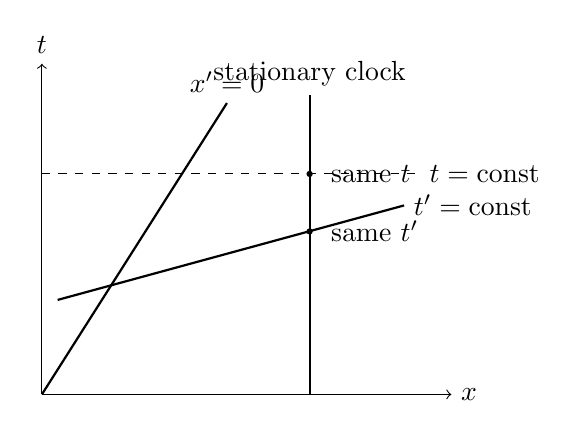
\begin{tikzpicture}[x=1cm,y=1cm]
\draw[->] (0,0) -- (0,4.2) node[above] {$t$};
\draw[->] (0,0) -- (5.2,0) node[right] {$x$};

\draw[thick] (0,0) -- (2.35,3.7) node[above] {$x'=0$};

\draw[dashed] (0,2.8) -- (4.8,2.8);
\node[right] at (4.8,2.8) {$t=\mathrm{const}$};

\draw[thick] (0.2,1.2) -- (4.6,2.4);
\node[right] at (4.6,2.4) {$t'=\mathrm{const}$};

\draw[thick] (3.4,0) -- (3.4,3.8);
\node[above] at (3.4,3.8) {stationary clock};

\fill (3.4,2.8) circle (0.04);
\fill (3.4,2.07) circle (0.04);

\node[right] at (3.55,2.8) {same \(t\)};
\node[right] at (3.55,2.07) {same \(t'\)};
\end{tikzpicture}
\caption{Relativity of simultaneity. The stationary observer compares clock readings on a horizontal slice \(t=\mathrm{const}\), while the moving observer compares them on a tilted slice \(t'=\mathrm{const}\). The two statements about ``the other clock'' therefore refer to different event pairs.}
\end{figure}

This is the lecture's resolution of the reciprocity puzzle. Moving clocks appear slow to stationary observers, and stationary clocks appear slow to moving observers, because the very notion of ``at the same time'' is frame-dependent.

\section{Twin Paradox, Ideal Clocks, and Accelerated Motion}

Having established that clocks measure proper time, Susskind turns to the twin paradox. Two twins are born at the same event. One stays at home on a vertical worldline. The other is shot outward at speed \(v\), turns around, and comes back. When they meet again, they compare everything that can function as a clock: wristwatches, heartbeats, beard growth, metabolic aging. The question is not which clock was more poetic. The question is which worldline accumulated more proper time.

Let the stay-at-home twin measure a time \(T\) on the outward leg and another \(T\) on the return leg. Then
\begin{equation}
\tau_{\mathrm{home}}=2T.
\end{equation}
For the traveling twin, the turning point has coordinates
\begin{equation}
x=vT, \qquad t=T.
\end{equation}
Therefore one leg contributes
\begin{align}
\tau_{\mathrm{leg}}^2 &= T^2-x^2 \\
&= T^2-v^2T^2 \\
&= (1-v^2)T^2,
\end{align}
so
\begin{equation}
\tau_{\mathrm{leg}}=T\sqrt{1-v^2}.
\end{equation}
The return leg contributes the same amount, hence
\begin{equation}
\tau_{\mathrm{travel}}=2T\sqrt{1-v^2}.
\end{equation}
Since \(1-v^2<1\), the traveling twin returns younger.

\begin{figure}[h]
\centering
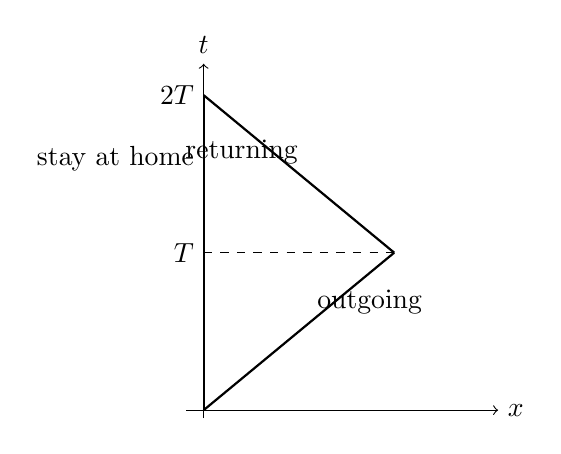
\begin{tikzpicture}[x=1.1cm,y=1cm]
\draw[->] (-0.2,0) -- (3.4,0) node[right] {$x$};
\draw[->] (0,-0.1) -- (0,4.4) node[above] {$t$};

\draw[thick] (0,0) -- (0,4);
\draw[thick] (0,0) -- (2.2,2);
\draw[thick] (2.2,2) -- (0,4);

\draw[dashed] (0,2) -- (2.2,2);

\node[left] at (0,2) {$T$};
\node[left] at (0,4) {$2T$};
\node[above right] at (1.2,1.1) {outgoing};
\node[above left] at (1.2,3.0) {returning};
\node[left] at (0,3.2) {stay at home};
\end{tikzpicture}
\caption{Twin paradox as a comparison of proper times along two worldlines: one straight and one broken. The clocks disagree because the paths through spacetime are different, not because the geometry is inconsistent.}
\end{figure}

Susskind is careful here. He does not leave the result as a mere slogan. The traveling twin is younger for the same reason that a broken path in geometry has a different length from a straight one. Minkowski geometry is unfamiliar, but it is still geometry.

\subsection{Question \& Answer}

\paragraph{Question.} Does the presence of acceleration destroy the argument? After all, the turnaround is not an inertial segment.

\paragraph{Answer.} No one should pretend the acceleration is absent. It is present, and it is one of the things that breaks the symmetry between the twins. But that does not spoil the proper-time calculation.

First, the sharp corner in the spacetime diagram is only an idealization. We may smooth it into a finite turnaround without changing the conclusion.

Second, the lecture introduces an additional physical assumption: the assumption of an ideal clock. A sufficiently small, well-built clock is taken to be insensitive to modest accelerations, so that it continues to tick off proper time. Then a curved worldline can be approximated by many short inertial segments, and one adds the proper times segment by segment:
\begin{equation}
\tau_{\mathrm{path}} \approx \sum_i \sqrt{\Delta t_i^2-\Delta x_i^2}.
\end{equation}
This is the spacetime analogue of computing the length of an ordinary curve by dividing it into many small straight pieces.

Susskind is explicit that this ideal-clock behavior is a physical assumption, not something proved from the Lorentz algebra alone. Small, faithful clocks may be engineered to withstand the relevant accelerations; big sloppy clocks may not. The geometry tells us what an ideal clock records.

The lecture then pushes the same issue into a more operational form. Instead of comparing final clock readings only, we imagine marking one-second intervals of proper time along both worldlines and sending light pulses back and forth. That way one asks not just what the clocks finally say, but how each observer actually receives the other's signals.

\section{Signals, Closed Spatial Loops, and Length Contraction}

Now the lecture leaves the purely geometrical comparison of two final clock readings and asks what each observer actually sees. Suppose the stay-at-home twin emits one light pulse every second of proper time, and the traveling twin does the same. On the outward leg the received pulses are stretched out; on the inward leg they become bunched together. Susskind explicitly identifies this as a Doppler-type effect, though he does not need the full formalism of relativistic Doppler shift to make the point.

What matters is the rhythm of reception. Early pulses arrive late and sparse; later pulses arrive fast and compressed. No pulses go missing. Each observer eventually receives all the pulses sent by the other, but at rates that reflect the relative motion. This operational discussion is important in the lecture because it keeps proper time from becoming a purely formal invariant. The geometry is read out by actual light signals.

A question about energy is raised at this point and then postponed. Susskind refuses to answer it too early. At this stage the lecture is about coordinates, clocks, and signals, not yet about the full relativistic bookkeeping of energy for accelerated observers.

\subsection{Question \& Answer}

\paragraph{Question.} What if one spatial direction were compact, so that an observer could move uniformly around a closed loop and return without the usual turn-around? Would the asymmetry survive?

\paragraph{Answer.} Here the lecture becomes exploratory and deliberately unfinished. Susskind first says that the asymmetry should survive, because the moving observer would discover a surprise: the same places would recur. But he then pulls back and refuses to give an unthought-out answer. The right way to preserve this beat is not to turn it into a polished theorem. It is to record the qualitative claim and the fact that the full geometry is postponed.

\begin{figure}[h]
\centering

\includegraphics[width=0.56\textwidth]{lecture_04_figure_04.png}
\caption{The later board during the compact-direction discussion. The left-board algebra is too fragmentary to transcribe safely, but the right-hand geometric sketch shows that the lecture had shifted into an asymmetry puzzle rather than a finished derivation.}
\end{figure}

\begin{figure}[h]
\centering
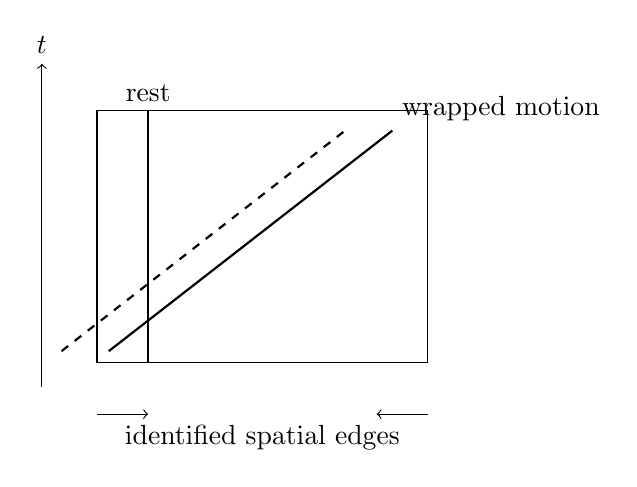
\begin{tikzpicture}[x=1cm,y=1cm]
\draw[->] (0,0) -- (0,4.1) node[above] {$t$};
\draw (0.7,0.3) rectangle (4.9,3.5);

\draw[->] (0.7,-0.35) -- (1.35,-0.35);
\draw[->] (4.9,-0.35) -- (4.25,-0.35);
\node at (2.8,-0.65) {identified spatial edges};

\draw[thick] (1.35,0.3) -- (1.35,3.5);
\node[above] at (1.35,3.5) {rest};

\draw[thick] (0.85,0.45) -- (4.45,3.25);
\draw[thick,dashed] (0.25,0.45) -- (3.85,3.25);
\node[above right] at (4.45,3.25) {wrapped motion};
\end{tikzpicture}
\caption{A cautious schematic reconstruction of the compact-direction question, drawn on an unwound strip. This is not a completed theorem from the lecture; it is only a clean rendering of the qualitative asymmetry being discussed.}
\end{figure}

Only after this detour does Susskind return to the next standard effect, and he does so with a piece of methodological advice strong enough to count as doctrine: when you want to understand a special-relativity problem, draw a picture.

Take a meter stick at rest in the unprimed frame. Its left end lies at \(x=0\), its right end at \(x=1\). As time passes, the rod sweeps out a ribbon in spacetime, bounded by two vertical worldlines. The question is: what length does the moving observer assign to that ribbon?

The answer begins with the meaning of measurement. A length in the moving frame is the separation of the rod's endpoints at the same instant of \emph{moving-frame} time. That is the local conceptual obstacle in this part of the lecture. One must not look at arbitrary points on the ribbon; one must intersect the ribbon with a single constant-\(t'\) slice.

The clean relation is
\begin{equation}
t-vx=\mathrm{const}
\end{equation}
for constant \(t'\) in units with \(c=1\). In particular, the slice through the origin with \(t'=0\) satisfies
\begin{equation}
t=vx.
\end{equation}
The lecture's spoken line wavers momentarily here, but this is the correct standard form. When the slice hits the right endpoint worldline \(x=1\), the corresponding unprimed time is therefore
\begin{equation}
t=v.
\end{equation}

\begin{figure}[h]
\centering
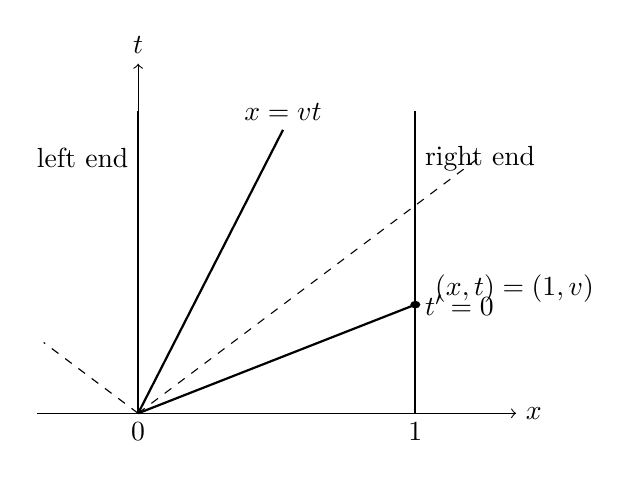
\begin{tikzpicture}[x=1.6cm,y=1.2cm]
\draw[->] (-0.8,0) -- (3.0,0) node[right] {$x$};
\draw[->] (0,0) -- (0,3.7) node[above] {$t$};

\draw[dashed] (0,0) -- (2.7,2.7);
\draw[dashed] (0,0) -- (-0.75,0.75);

\draw[thick] (0,0) -- (0,3.2);
\draw[thick] (2.2,0) -- (2.2,3.2);

\node[below] at (0,0) {$0$};
\node[below] at (2.2,0) {$1$};

\draw[thick] (0,0) -- (1.15,3.0);
\node[above] at (1.15,3.0) {$x=vt$};

\draw[thick] (0,0) -- (2.2,1.15);
\node[right] at (2.2,1.15) {$t'=0$};

\fill (2.2,1.15) circle (0.04);
\node[right] at (2.28,1.32) {$(x,t)=(1,v)$};

\node[left] at (0,2.7) {left end};
\node[right] at (2.2,2.7) {right end};
\end{tikzpicture}
\caption{Length contraction from the spacetime picture Susskind insists on drawing. The rod is at rest in the unprimed frame, so its endpoints trace a vertical ribbon. The moving observer measures the rod by slicing that ribbon with a constant-\(t'\) line.}
\end{figure}

Because the separation from the origin to the selected endpoint is now space-like, it is cleaner to reverse the sign of the invariant interval and speak of the squared proper distance:
\begin{equation}
x'^2-t'^2 = x^2-t^2.
\end{equation}
On the chosen slice, \(t'=0\). At the selected endpoint, \(x=1\) and \(t=v\). Therefore
\begin{equation}
x'^2 = 1-v^2.
\end{equation}
Equivalently, in the lecture's board language one may write
\begin{equation}
-x'^2 = v^2-1,
\end{equation}
which is the same statement with the signs not yet cleaned up. Either way the conclusion is
\begin{equation}
x'=\sqrt{1-v^2}.
\end{equation}
Thus a rod of rest length \(1\) is seen in the moving frame to have length
\begin{equation}
L'=\sqrt{1-v^2}.
\end{equation}
For a general rest length \(L\),
\begin{equation}
L' = L\sqrt{1-v^2}
\end{equation}
in units with \(c=1\), or
\begin{equation}
L' = L\sqrt{1-\frac{v^2}{c^2}}
\end{equation}
when \(c\) is restored.

This is the companion to time dilation. Time dilation came from following a moving worldline and comparing elapsed proper time. Length contraction comes from slicing a stationary ribbon by the moving observer's simultaneity plane. Both are consequences of the same Lorentz mixing of space and time.

The lecture's final operational payoff is immediate. In the astronaut's frame the distance between distant stars is Lorentz-contracted, so a long trip may take a short proper time without anything moving faster than light. The stars are not seen to outrun light; they are simply seen at a reduced spatial separation in the moving frame.

\section{Summary}

The lecture begins with Galileo on purpose. In the Galilean picture the moving origin tilts, but time slices remain common to everyone. Einstein's correction changes exactly that point: \(x\) and \(t\) mix, the light cone is preserved, and the invariant quantity is not \(x^2+y^2\) but \(t^2-x^2-y^2-z^2\).

From there the lecture unfolds in a strict order. First we reinterpret the Lorentz transformation as a squeeze along null directions. Then we identify the invariant interval. Then we define proper time and recognize it as the time read by a moving clock. Time dilation follows from evaluating that invariant on the worldline \(x=vt\). The reciprocity puzzle is resolved by relativity of simultaneity. The twin paradox is resolved by comparing proper times along different paths, with the ideal-clock assumption made explicit. Signal exchange gives the operational picture. A compact-direction asymmetry is raised but deliberately left provisional. Only after that does Susskind return to length contraction, again by drawing the spacetime picture first.

What remains after all the formulas is really a method. Draw the diagram. Identify the invariant. Ask which events are being compared. Then let the geometry tell you what clocks, rods, and signals will do.